%%%%%%%%%%%%%%%%%%%%%%%%%%%%%%%%%%%%%%%%%
% Short Sectioned Assignment
% LaTeX Template
% Version 1.0 (5/5/12)
%
% This template has been downloaded from:
% http://www.LaTeXTemplates.com
%
% Original author:
% Frits Wenneker (http://www.howtotex.com)
%
% License:
% CC BY-NC-SA 3.0 (http://creativecommons.org/licenses/by-nc-sa/3.0/)
%
%%%%%%%%%%%%%%%%%%%%%%%%%%%%%%%%%%%%%%%%%

%----------------------------------------------------------------------------------------
%	PACKAGES AND OTHER DOCUMENT CONFIGURATIONS
%----------------------------------------------------------------------------------------

\documentclass[paper=a4, fontsize=11pt]{scrartcl} % A4 paper and 11pt font size

\usepackage[T1]{fontenc} % Use 8-bit encoding that has 256 glyphs
\usepackage{fourier} % Use the Adobe Utopia font for the document - comment this line to return to the LaTeX default
\usepackage[english]{babel} % English language/hyphenation
\usepackage{amsmath,amsfonts,amsthm} % Math packages
\usepackage[utf8]{inputenc}
\usepackage{lipsum} % Used for inserting dummy 'Lorem ipsum' text into the template

\usepackage{sectsty} % Allows customizing section commands
\allsectionsfont{\centering \normalfont\scshape} % Make all sections centered, the default font and small caps

\usepackage{yfonts,color}
\usepackage{graphicx}

\usepackage{fancyhdr} % Custom headers and footers
\pagestyle{fancyplain} % Makes all pages in the document conform to the custom headers and footers
\fancyhead{} % No page header - if you want one, create it in the same way as the footers below
\fancyfoot[L]{} % Empty left footer
\fancyfoot[C]{} % Empty center footer
\fancyfoot[R]{\thepage} % Page numbering for right footer
\renewcommand{\headrulewidth}{0pt} % Remove header underlines
\renewcommand{\footrulewidth}{0pt} % Remove footer underlines
\setlength{\headheight}{13.6pt} % Customize the height of the header

\numberwithin{equation}{section} % Number equations within sections (i.e. 1.1, 1.2, 2.1, 2.2 instead of 1, 2, 3, 4)
\numberwithin{figure}{section} % Number figures within sections (i.e. 1.1, 1.2, 2.1, 2.2 instead of 1, 2, 3, 4)
\numberwithin{table}{section} % Number tables within sections (i.e. 1.1, 1.2, 2.1, 2.2 instead of 1, 2, 3, 4)

\newcommand{\parta}{\emph{a)\,}}
\newcommand{\partb}{\emph{b)\,}}
\newcommand{\partc}{\emph{c)\,}}
\newcommand{\partd}{\emph{d)\,}}
\newcommand{\parte}{\emph{e)\,}}
\newcommand{\partf}{\emph{f)\,}}
\newcommand{\m}{\mathrm}
\newcommand{\ddx}{\frac{\mathrm{d}}{\mathrm{dx}}}
\newcommand{\dydx}{\frac{\mathrm{d}y}{\mathrm{d}x}}
\newcommand{\dydydxdx}{\frac{\mathrm{d}^2y}{\mathrm{d}x^2}}
\newcommand{\ddt}{\frac{\mathrm{d}}{\mathrm{dt}}}
\newcommand{\fx}{\m{f}(x)}
\newcommand{\gx}{\m{g}(x)}
\newcommand{\hx}{\m{h}(x)}
\newcommand{\dx}{\m{d}x}
\newcommand{\fy}{\m{f}(y)}
\newcommand{\gy}{\m{g}(y)}
\newcommand{\hy}{\m{h}(y)}
\newcommand{\dy}{\m{d}y}

\setlength\parindent{0pt} % Removes all indentation from paragraphs - comment this line for an assignment with lots of text

%----------------------------------------------------------------------------------------
%	TITLE SECTION
%----------------------------------------------------------------------------------------

\newcommand{\horrule}[1]{\rule{\linewidth}{#1}} % Create horizontal rule command with 1 argument of height

\title{	
\normalfont \normalsize 
\textsc{} \\ [25pt] % Your university, school and/or department name(s)
\horrule{0.5pt} \\[0.4cm] % Thin top horizontal rule
\huge Pressure-law Broad Line Region with $s=0$ (constant nH)\\ % The assignment title
\horrule{2pt} \\[0.5cm] % Thick bottom horizontal rule
}

%\author{Daniel Lawther (unclellama@gmail.com)} % Your name

%\date{\normalsize\today} % Today's date or a custom date

\begin{document}
\date{}
\maketitle

\section{Setting up the $s=0$ pressure-law BLR model}

For a pressure-law BLR cloud distribution we have

\begin{equation*}
P(r)\propto r^{-s}.
\end{equation*}

For this first investigation we are looking at a constant-pressure model, i.e., $s=0$. This leads to the following relations (e.g., Rees+1989, Goad+1993):\\

Cloud gas density is constant for $s=0$\footnote{Assuming constant temperature - how much do real BLR deviate from this?}:

\begin{equation*}
n_H(r)\propto r^{-s}
\end{equation*}

The ionization parameter $U$ at ionizing photon-counting flux $Q(H)$ and hydrogen number density $N$:

\begin{equation*}
U=Q(H)/(4\pi r^2cN)
\end{equation*}

This has the $r$-dependence:

\begin{equation*}
U(r)\propto r^{s-2}
\end{equation*}

(this is constant as a function of radius for the $s=2$ case, which we want to investigate later!)\\

Surface area per cloud $A_c$ is proportional to cloud radius squared. Mass conservation for radial motion of individual clouds requires that $R_c^3n_H$ is constant:

\begin{equation*}
A_c(r) \propto R_c^2(r) \propto r^{2s/3}
\end{equation*}

And the column density of the clouds depends on the gas density and cloud radius:

\begin{equation*}
N_{col}(r)\propto R_cN_H
\end{equation*}

According to the above, both the column density $N_{col}$ and the cloud density $n_H$ are constant for $s=0$. Therefore, for the constant-pressure case, we work with constant-$n_H$ slices through \emph{Cloudy} grids generated at a given $N_{col}$.

\subsection{Getting the normalization for $A_c(r)n_c(r)$}

The total luminosity for a BLR line is given by the integral

\begin{equation*}
L=4\pi\int_{r_{in}}^{r_{out}}\epsilon(r)A_c(r)n_c(r)r^2dr
\end{equation*}

Here, $\epsilon$ denotes the line emissivity per cm$^2$ of cloud surface, and $n_c(r)$ is the number density of clouds. Assuming a power-law distribution $n_c\propto r^{-p}$, and virial motion of the clouds ($v(r)\propto r^{-1/2}$), mass conservation implies the following relation for the differential covering factor:

\begin{equation*}
dC(r) \propto A_c(r)n_c(r) dr \propto r^{2s/3-3/2} dr
\end{equation*}

This relation allows us to determine a normalization constant for the total line-emitting surface of the clouds (the volume integral of $A_c(r)n_c(r)$), for a given total covering factor of the central source (the solid angle $\Omega$ covered by a single cloud `as seen from the source' goes as $d\Omega=dA_c/r^2$). The normalization factor can be found analytically for a given $s$, or determined numerically - after some debugging, both approaches agree! The luminosity integral becomes:

\begin{equation*}
L=4\pi k\int_{r_{in}}^{r_{out}}\epsilon(r)r^{2s/3+1/2}dr
\end{equation*}

where $k$ is the scaling constant found by integrating over $dC$.\\

\subsection{Getting the integrated line luminosities}

We have a grid of \emph{Cloudy} models for each emission line, providing the emissivity $\epsilon$, as a function of $n_H$, $N_{col}$, and the ionizing flux $\Phi(H)$. For a given source luminosity and SED shape, the $\Phi$ axis in these grids can be converted into a radial axis, allowing the evaluation of the integral $L$. The resulting line luminosities thus depend on $n_H$, $N_{col}$, the ionizing continuum SED, the inner and outer BLR radii, and the total covering fraction of the BLR. The dependence of $L$ on $r_{in}$ is strong for $s=0$, in the sense that smaller inner radii lead to smaller integrated luminosities - this is due to the model distributing most of the clouds close to the inner radius, where they become overionized if the inner radius is small.\\

To start with we assume total coverage of the continuum source, so as to obtain an upper limit on the line luminosities attainable. We assume an inner BLR radius of 1 lightday (as suggested by RM monitoring), and an outer radius of 140 lightdays (as set by the dust sublimation radius for our adopted source luminosity).

\section{Line luminosities and effective radii as a function of $n_H$}

\subsection{Matching the observed line luminosities}

Figure \ref{fig:lnh}, top left panel, shows the line luminosities produced for the Ly$\alpha$, \textsc{c IV}, and H$\beta$ emission lines, as a function of $n_H$, for $N_{col}=10^{23}$ cm$^{-2}$. (We find that, for intermediate values of $n_H$, the resulting luminosities are not strongly sensitive to $N_{col}$ over the range $22\le\log(N_c)\le24$.)\\ 

Ideally we want these luminosities to be larger than the observed, dereddened line luminosities, as this will allow us to assume a smaller covering fraction - our model does not take BLR self-shadowing into account, so becomes unreliable at high covering fractions. At $\log n_H\sim11$, our $s=0$ model can exceed the observed broad-line luminosities for Ly$\alpha$ and \textsc{c IV}, but has trouble reproducing the observed H$\beta$ flux.

 

\begin{figure}
	\centering
	\includegraphics[width=0.49\linewidth]{L_nH}
	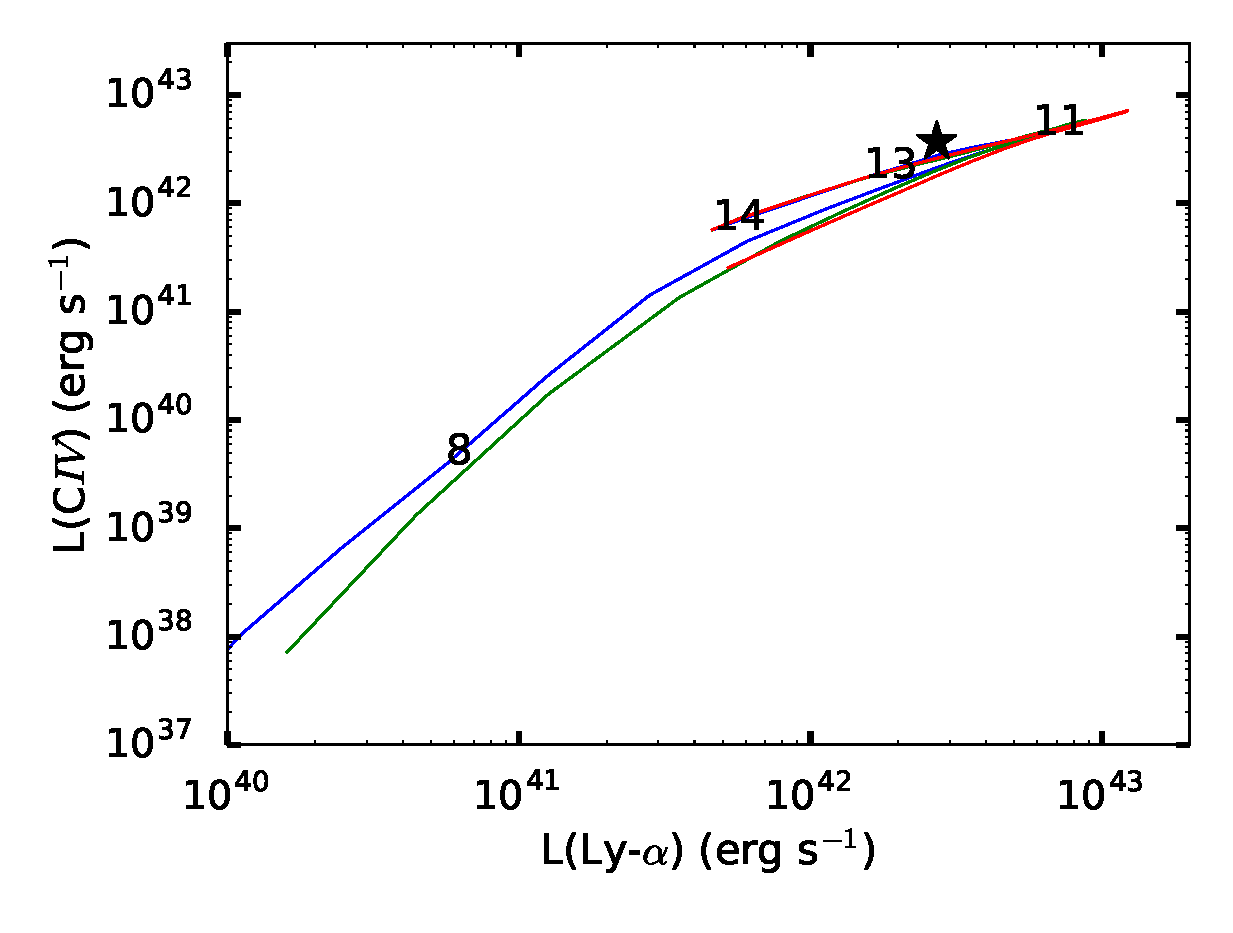
\includegraphics[width=0.49\linewidth]{lineL_civ_rin1}
	\includegraphics[width=0.49\linewidth]{lineL_hbeta_rin1}
	\includegraphics[width=0.49\linewidth]{RL_nH}
	\caption{Top left: line luminosities integrated between the inner and outer BLR radius. Top right: Ly$\alpha$ versus \textsc{c IV} luminosity for a range of $n_H$; the green data point denotes the observed line luminosity ratio (after Galactic dereddening and subtraction of the narrow-line component). The superimposed numbers show the value of $\log n_H$ at that point on the curve. Bottom left: Ly$\alpha$ versus H$\beta$ luminosity. Bottom right: luminosity-weighted effective BLR radii, in units of lightdays, as a function of $n_H$.}
	\label{fig:lnh}
\end{figure}

\subsection{Effective radii of the line-emitting regions}

Figure \ref{fig:lnh}, bottom right panel, shows the effective radii in light-days, using luminosity-weighting. I.e., the radius is weighted towards the regions that produce more of the total luminosity. For $n_H<~10$, the luminosity-weighted radii of the three lines are very similar - in a constant-pressure BLR with clouds below this density, the three lines would appear to be produced at the same radii.\\

In Figure \ref{fig:em-weghted} we compare the luminosity-weighted radii with resposivity-weighted radii. The responsivities $\eta(r)$ are defined as $\eta=d\log(\epsilon(r))/d\log(\Phi(r))$. Thus, $\eta=1$ implies that the equivalent width of a line is constant for a small change in the ionizing flux level. The responsivity-weighted radii are more relevant to RM campaigns, as they give the radius at which we will preferentially see emission line response to continuum variations. For these emission lines, we tend to see larger emissivity-weighted radii compared to luminosity-weighted, i.e, the gas at larger radii responds more strongly to the continuum flux.\\ 

Note: at very low densities $\log n_H<8$, the responsivities are negative for much of the inner region of the BLR - and, as the BLR is sparsely sampled in $\Phi$ here, there are likely numerical issues with my code, giving strongly negative responsivity-weighted radii here - need to look into this more!

\begin{figure}
	\centering
	\includegraphics[width=0.49\linewidth]{RL_nH}
	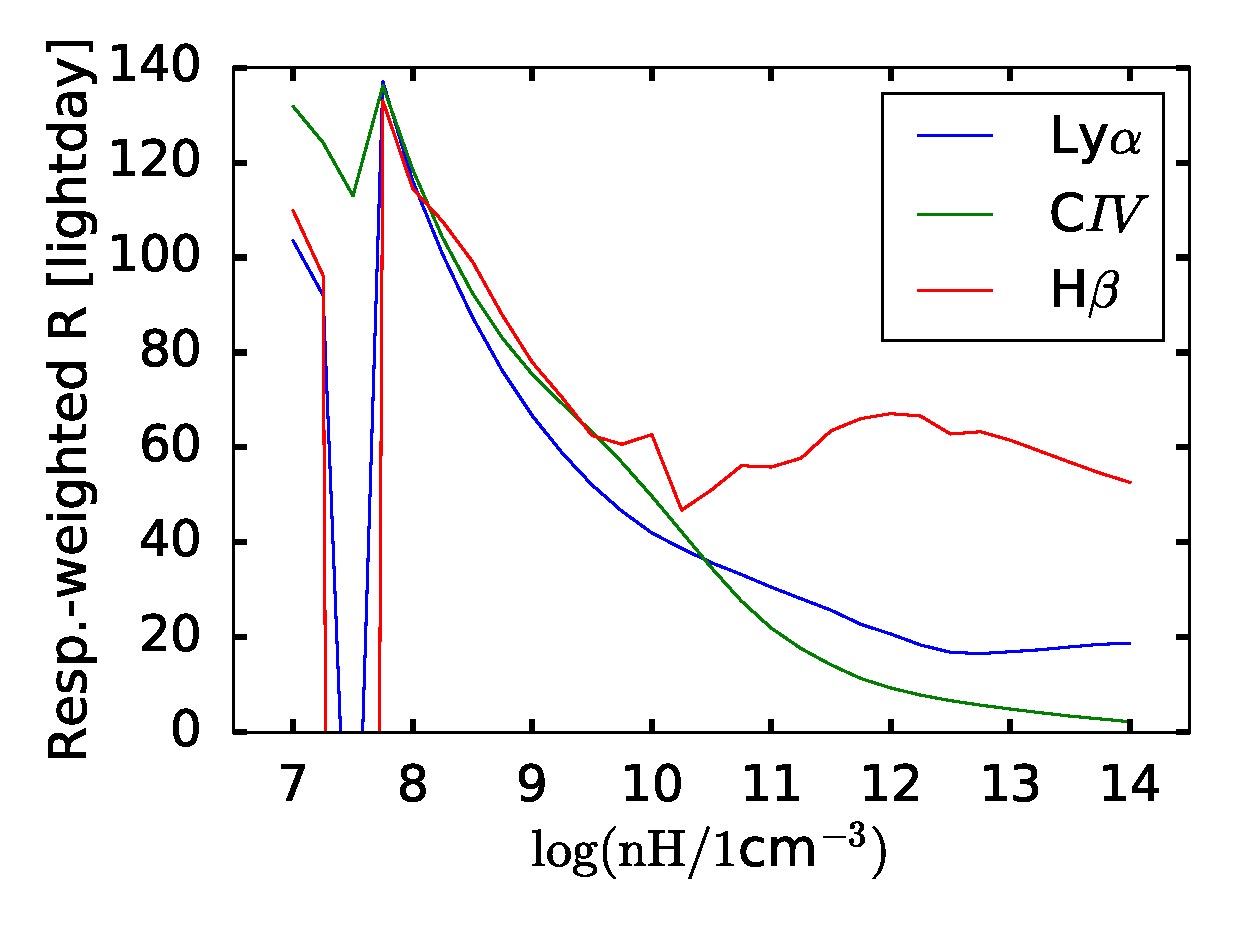
\includegraphics[width=0.49\linewidth]{RR_nH}
	\caption{Effective BLR radii as a function of $n_H$, using luminosity-weighting (left panel) and responsivity-weighting (right panel).}
\label{fig:em-weghted}
\end{figure}

\section{Diffuse continuum for nH = 11}

The `diffuse continuum' is the continuum emission produced by the BLR clods themselves. As we found that models with $\log n_H\sim11$ produce enough luminosity to roughly match or exceed the observed emission line levels, we now examine the diffuse continuum produced for the pressure law BLR with constant density $\log n_H=11$. The \emph{Cloudy} grids provided include the diffuse continuum emissivity in several wavelength bands, again as a function of $n_H$, $Phi(H)$, and $N_{col}$; we integrate the total luminosity of each of these bands in the same way as for the emission lines, providing a spectrum of $\nu L_{\nu}$ as a function of wavelength for the diffuse continuum (Figure \ref{fig:cont}, top left). Note the strong Balmer continuum feature at wavelengths below the Balmer break $\sim3646$ Ang.\\

Assuming a power-law form for the nuclear continuum, extrapolated from the continuum luminosity at 1215 Ang, we calculate the ratio of diffuse continuum to total (nuclear + diffuse) as a function of wavelength. The diffuse continuum exceeds the nuclear continuum emission near the Balmer break (Figure \ref{fig:cont}, top right). As for the emission lines, we can find the luminosity-weighed and emissivity-weighted radii for the diffuse continuum (bottom left panel), and the effect of diluting the diffuse continuum emission with the appropriate fraction of nuclear-continuum light (assuming the latter is a point-source). It is interesting that these models predict elevated continuum delays near the Balmer break, relative to the $R\propto\lambda^{-4/3}$ dependence suggested for emission from the surface of an accretion disk.

\begin{figure}
	\centering
	\includegraphics[width=0.49\linewidth]{diff_cont_lumin}
	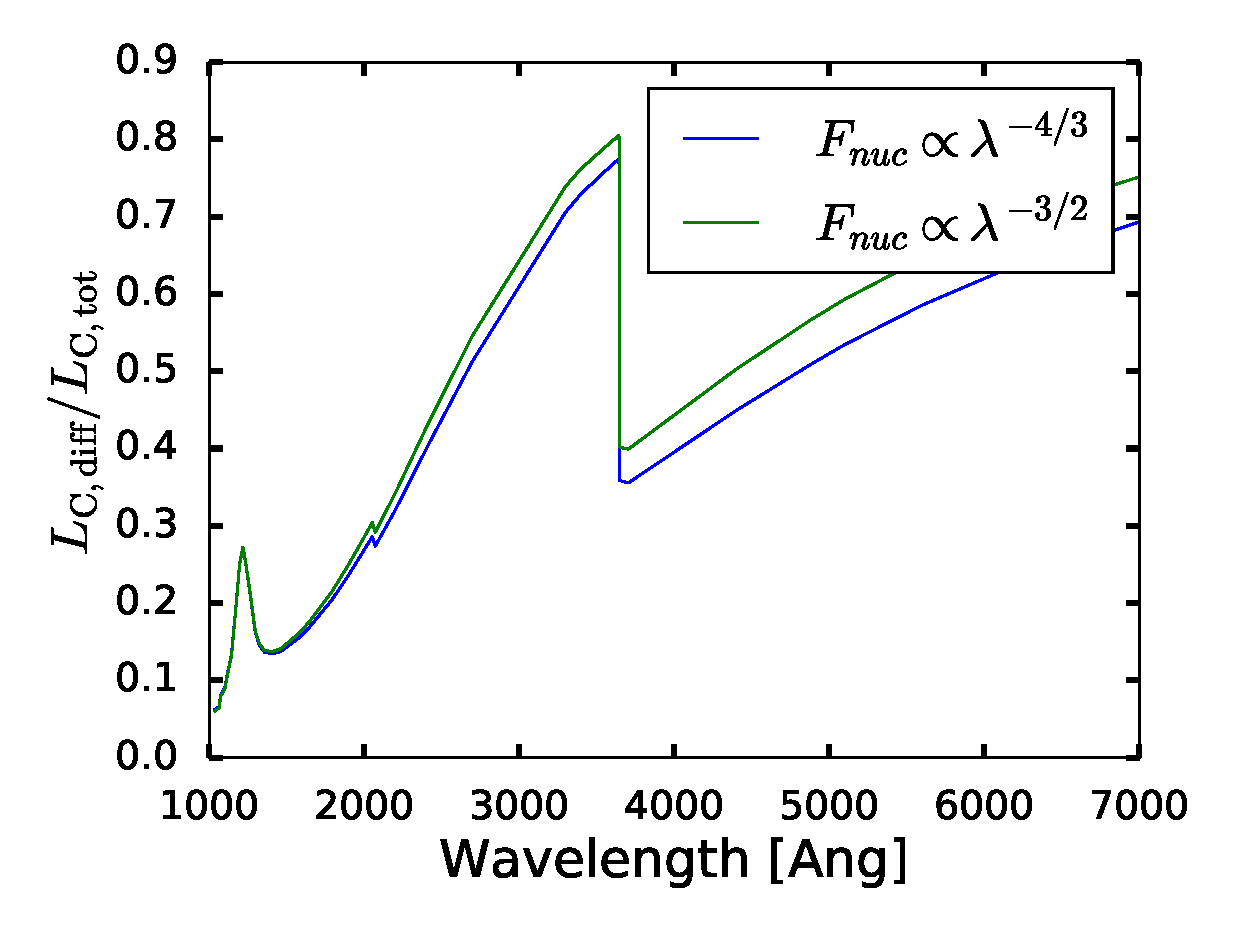
\includegraphics[width=0.49\linewidth]{cont_frac}
	\includegraphics[width=0.49\linewidth]{diff_cont_R}
	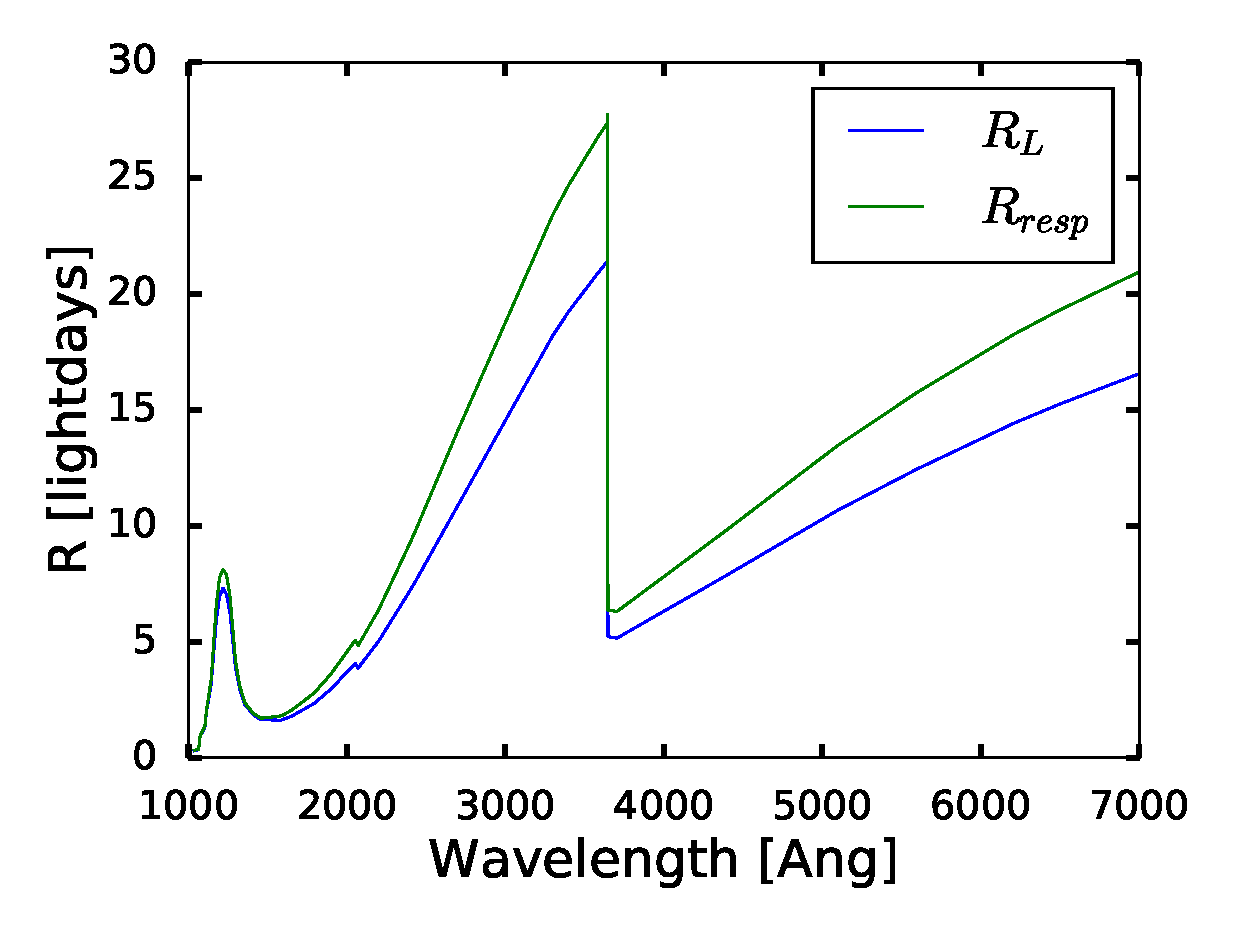
\includegraphics[width=0.49\linewidth]{diluted_cont_R}
	\caption{Top left: diffuse BLR continuum $\nu F_{nu}$ as a function of wavelength. Top right: Ratio of diffuse continuum to total (nuclear + diffuse) continuum luminosity, as a function of wavelength. Bottom left: Effective radii for the diffuse continuum. Bottom right: effective radii for the total + diffuse continua, assuming that the nuclear continuum is a point source at all wavelengths.}
	\label{fig:cont}
\end{figure}

\end{document}